% Clase del documento (class)
\documentclass[a4paper,12pt]{article}
%\documentclass[a4paper,10pt]{scrartcl}

%-------------------------------------------------------------------------------
% Preámbulo del documento (preamble)
% Paquetes incluidos
%\usepackage[latin1]{inputenc}
\usepackage[utf8]{inputenc}
\usepackage[T1]{fontenc}
\usepackage[spanish]{babel}
\usepackage{graphicx}
\usepackage[nottoc, notlot, notlof, notindex]{tocbibind}	% Incluye la bibliografía (referencias) en el índice (tabla de contenidos).
% Las opciones son:
% notoc -> no incluir el índice general
% notlot -> no incluir el índice de tablas
% notlof -> no incluir el índice de figuras
% notindex -> no incluir el índice alfabético
% notbib -> no incluir la bibliografía

% Formato de los márgenes
\usepackage{anysize}
\marginsize{2.5cm}{2.5cm}{2.5cm}{2.5cm}

% Título, autor, fecha, etc.
\title{Pronóstico de Partidos de Fútbol:\\Documentación Técnica}
\author{José Miguel Horcas Aguilera}
\date{3/06/2010}

% Información para el pdf.
\pdfinfo{%
  /Title    ()
  /Author   ()
  /Creator  ()
  /Producer ()
  /Subject  ()
  /Keywords ()
}

%---------------------------------------------------------------------------------
% Cuerpo del documento (document body)
\begin{document}
%\renewcommand{\labelitemi}{$\bullet$ }
\renewcommand{\figurename}{Figura}
\maketitle

\begin{abstract} % Resumen
Este documento describe los aspectos técnicos de la aplicación realizada para el trabajo práctico de la asignatura \textit{Amplicación de Ingeniería del Conocimiento}.
Se explican las fuentes de conocimiento empleadas y se detalla tanto el diseño de la red bayesiana usada como los detalles más importantes de la aplicación en sí misma.
\end{abstract}
\tableofcontents
\newpage

\section{Dominio de aplicación}
\label{sec:dominio}
\par
Predicción de resultados futbolísticos mediante una red bayesiana.
\\
Hay numerosas variables que pueden afectar al resultado de un partido de fútbol:
equipos, jugadores, entrenadores, tácticas, árbitros, bajas, cansancio,
condiciones meteorológicas, objetivos de cada equipo, resultados anteriores,\dots
y muchísimas variables más.
\\
Teniendo en cuenta toda esta información se diseña un Sistema Basado en el Conocimiento (SBC) que usa el razonamiento aproximado para predecir de forma realista el resultado de un partido de fútbol.

\subsection{Casos de uso}
\par
La función principal de la aplicación es predecir el resultado de un partido de fútbol en términos de número de goles marcados por cada equipo.
Como resultado presenta además las probabilidades que tienen ambos equipos de ganar, empatar o perder, así como las probabilidades de los distintos resultados que se puedan dar.
\par
La aplicación permite al usuario introducir la información necesaria a través de un sencillo formulario con preguntas referentes al partido y a los equipos enfrentados.

\section{Fuentes de conocimiento empleadas}
\label{sec:conocimiento}
\par
En el desarrollo de la aplicación se han empleado las redes bayesianas como técnica de razonamiento aproximado.
La decisión de escoger esta técnica en lugar de la lógica difusa es el hecho de que conocer el resultado de un partido de fútbol antes de jugarlo representa una situación de incertidumbre del mundo real.
Y dado que la incertidumbre se representa basándose en la teoría de la probabilidad, las redes bayesianas nos permiten realizar este tipo de inferencias predictivas.
\par
Aunque, como veremos más adelante, en nuestra aplicación manejamos información imprecisa con algunos nodos de la red.
Para no complicar en exceso el diseño no entraremos en terreno de la lógica difusa para resolver estas situaciones.

  \subsection{Proceso de extracción de la información}
\par
La información necesaria para el SBC no ha podido ser extraída directamente de un experto, debido principalmente a la falta de medios.
Sin embargo, se han utilizado diferentes libros y guías editados por expertos del mundo del fútbol para extraer toda la información necesaria \cite{GM0910}.
Se ha obtenido información de las posibles variables que pueden intervenir en el resultado de un partido de fútbol, así como las relaciones entre ellas y los valores que pueden tomar.
Además, el hecho de disponer de estas fuentes de información ricas en datos estadísticos facilita la asignación de las probabilidades a los nodos de la red.

\section{Razonamiento del sistema}
\label{sec:razonamiento}
El razonamiento del sistema se basa en una red bayesiana que nos permite hacer inferencias predictivas sobre el resultado de un partido de fútbol.
El fichero \textit{redFutbol.xdsl} contiene la red bayesiana del SBC.

  \subsection{Principales decisiones de diseño}
\par
La aplicación dispone de una red bayesiana diseñada con el programa GeNIe.
A partir de esta red bayesiana se ha diseñado una interfaz gráfica de usuario en Java apropiada para proporcionarle los datos necesarios.
Para ello se ha usado la biblioteca jSMILE que nos permite trabajar con la red en el lenguaje de programación Java.

	\subsubsection{La red bayesiana}
\par
La red bayesiana con la que trabaja el sistema consta de 95 nodos que representan las variables que pueden influir en el resultado de un partido de fútbol.
Estas variables serán en su mayoría binarias, pero hay otras muchas variables con tres o cuatro valores.
Incluso hay variables con 7 valores para representar el número de goles que marcan los equipos; y una variable con 16 valores para el resultado exacto del partido,
aunque para esa variable será fácil asignar las probabilidades, pues serán directamente 0 ó 1.
\\Estos nodos se conectan entre sí por arcos que representan las relaciones de influciencia causal existentes entre las variables.
En total hay 143 arcos en la red, que aunque puedan parecer pocos para el número de nodos con los que cuenta la red,
el hecho de que haya muchos nodos con más de dos posibles valores hace que el número de posibilidades aumente rápidamente.
\par
Las principales variables ocultas, objetos de interés, que no pueden ser observables directamente son:
\begin{itemize}
 \item El número de goles que marcará cada equipo en el partido.
 \item El resultado del partido en función del número de goles marcado por cada equipo,
 \item y el signo del partido, que como es lógico dependerá del resultado del partido.
\end{itemize}
La figura~\ref{fig:nodosObjetivos} muestra estas variables objetivos.
\begin{figure}[h]
 \begin{center}
  \includegraphics[scale=0.4]{nodosObjetivos.eps}
\caption{Principales variables ocultas, objetos de interés.}
\label{fig:nodosObjetivos}
 \end{center}
\end{figure} 
\\
A partir de estos objetivos se construye una inmensa red en la que podemos distinguir varias partes bien diferenciadas:
\\Por un lado se tiene la información general sin tener en cuenta datos sobre los equipos.
\\Por otro lado hay dos partes similares pero independientes entre sí que se refieren a datos propios de cada equipo,
lo que significa que habrá nodos y relaciones repetidos para representar la información concreta de cada uno.
Estas dos partes no serán exáctamente iguales, ya que existen variables que influyen unicamente sobre un equipo;
como por ejemplo el viaje que debe realizar el equipo visitante desde su ciudad hasta la ciudad del equipo local.
\\Por último hay nodos que representan información común sobre los dos equipos y que pueden, o no, estar conectados con las demás partes de la red.
La figura~\ref{fig:esquemaRed} muestra un esquema básico con esta división de la información para la red bayesiana.
\begin{figure}[h]
 \begin{center}
  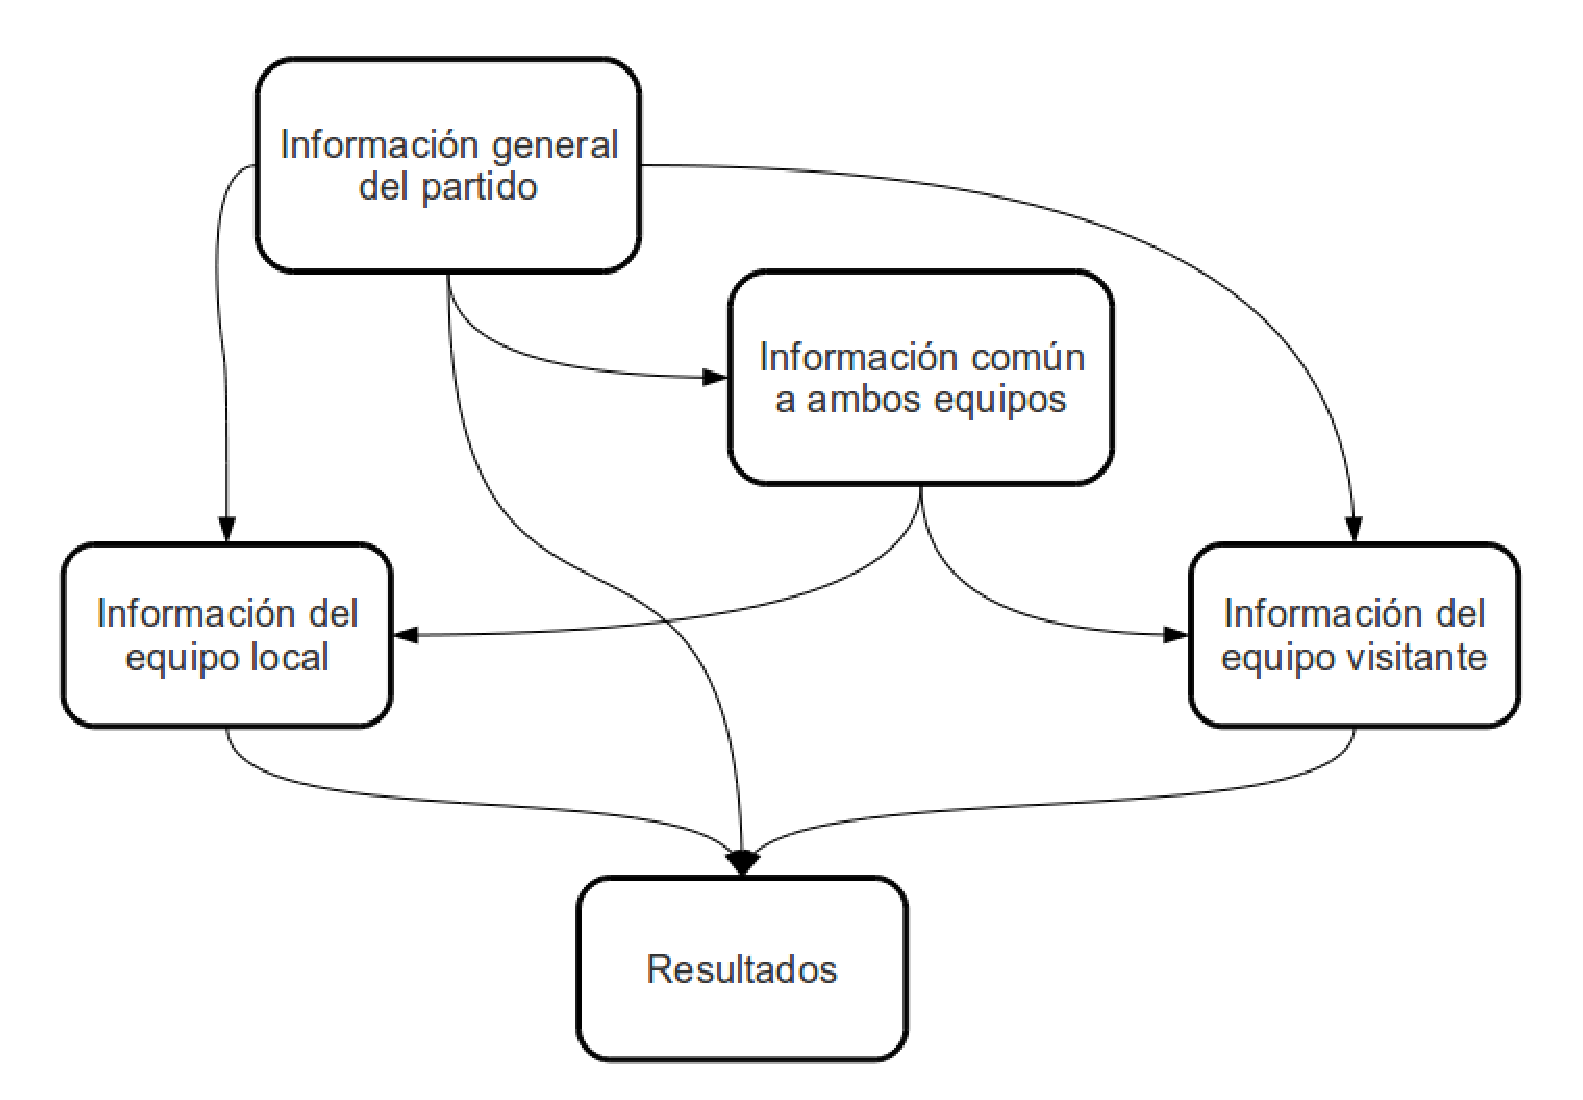
\includegraphics[scale=0.4]{esquemaRed.eps}
\caption{Esquema básico con las diferentes partes de la red bayesiana.}
\label{fig:esquemaRed}
 \end{center}
\end{figure} 

 \subsubsection{Información imprecisa}
\par
Algunos nodos representan variables con valores difusos; por ejemplo para la varible \textit{Distancia entre ciudades},
sus posibles valores son: \textit{corta}, \textit{media} ó \textit{larga}.
Esto nos permite aplicar en este punto la lógica difusa para instanciar esta variable,
aunque en nuestra aplicación y para simplificar el diseño omitiremos este aspecto,
pasando la responsabilidad de tratar con la información imprecisa al usuario, que será el encargado de decidir si la distancia entre las ciudades de los equipos es corta, media o larga.

  \subsubsection{Parámetros de la red}
\par
Los parámetros de la red se han proporcionado a mano directamente sobre la red usando el programa GeNIe.
La mayoría de las probabilidades de los diferentes nodos se han obtenido a partir de los datos estadísticos disponibles en la fuentes de extracción de la información, \cite{GM0910}.
Aunque estos parámetros los podía haber aprendido sola la red,
el trabajo que supone adaptar los datos disponibles al formato adecuado y la gran cantidad de nodos que contiene la red descartan esta opción.
Además, hay nodos para los cuales las probabilidades han tenido que inventarse.

\subsubsection{La interfaz gráfica}
\par
La aplicación consta de una sencilla interfaz gráfica diseñada en Java.
Ésta permite al usuario introducir la información necesaria de forma cómoda,
ocultando todo el proceso de razonamiento de la red bayesiana.
\par
Para el diseño de la interfaz gráfica se ha seguido el patrón de diseño MVC (Modelo-Vista-Controlador).
Este patrón separa, por un lado, los datos y la funcionalidad de la aplicación (el modelo)
de su representación (la vista) y de la forma en que se interactúa con el modelo a través de la vista (el controlador).
En la figura~\ref{fig:mvc} se muestra las relaciones básicas existentes entre las tres entidades del patrón MVC.
Con estas relaciones básicas, el controlador conoce la vista y el modelo, y es el encargado de realizar todas las acciones requeridas.
\begin{figure}[h]
 \begin{center}
  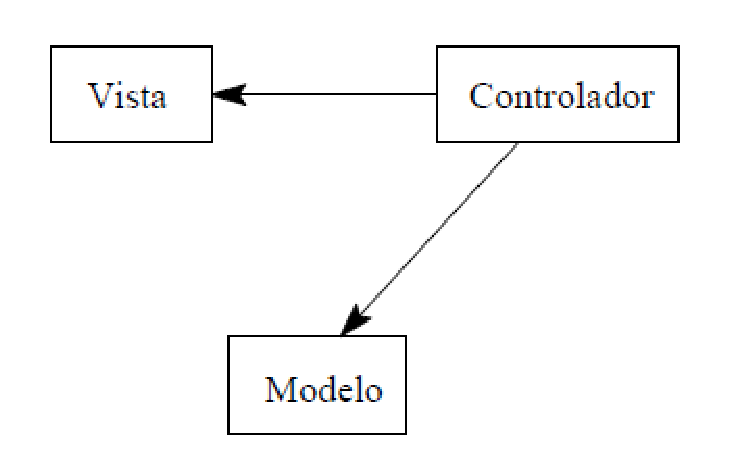
\includegraphics[scale=0.5]{mvc.eps}
\caption{Relaciones entre las entidades del patrón de diseño MVC.}
\label{fig:mvc}
 \end{center}
\end{figure} 

\par
El modelo de nuestra aplicación es la red bayesiana,
que representaremos por medio de una clase: \texttt{RedBayesiana}.
Esta clase usa el paquete jSMILE para realizar inferencias con la red.
Los métodos de la clase \texttt{RedBayesiana} nos ofrecen una interfaz más amigable que la proporcionada directamente por jSMILE para el uso de nuestra red.
En la figura~\ref{fig:diagramaModelo} podemos ver el diagramas de clases de nuestro modelo.
\begin{figure}[h]
 \begin{center}
  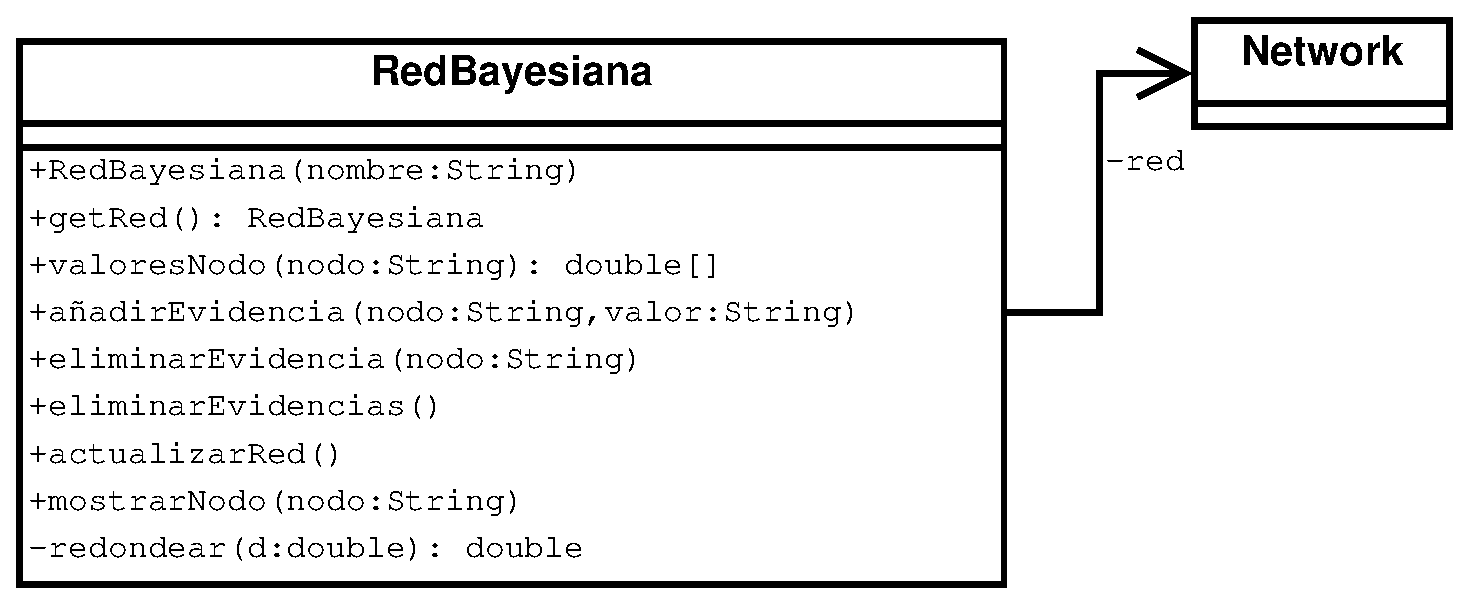
\includegraphics[scale=0.5]{diagramaModelo.eps}
\caption{Diagrama de clases del modelo de la aplicación.}
\label{fig:diagramaModelo}
 \end{center}
\end{figure}

\par
La vista cuenta con una ventana con cuatro pestañas.
Las tres primeras pestañas son formularios para la introducción de la información por parte del usuario.
La última pestaña muestra los resultados del pronóstico.
\par
El controlador es el encargado de actuar cuando el usuario decide realizar una acción sobre un elemento visible y activo de la vista.
En nuestra aplicación el controlador sólo va a intervenir en caso de que el usuario seleccione la última pestaña de la vista, que muestra los resultados.
En ese caso, el controlador recoge toda la información proporcionada por el usuario en las demás pestañas de la vista,
se la pasa al modelo para realizar el razonamiento sobre la red,
y a continuación actualiza la vista con los resultados devueltos por el modelo.
\\
Destacar que el usuario puede realizar todos los cambios que desee sobre la información proporcionada cada vez que lo necesite,
actualizándose los resultados cada vez que se active la última pestaña.

\section{Pruebas}
\par
El funcionamiento del SBC se ha ido probando poco a poco conforme se ha ido desarrollando.
Así, una vez construida la red y proporcionados los parámetros de todas las variables,
se probó la eficacia de la red utilizando un caso real:
el pronóstico de los resultados de los partidos correspondientes a la última jornada de la liga española de primera división\footnote{Jornada nº 38 de la temporada 2009/2010 (15 y 16 de mayo) en la que se decidía el título de liga y el descenso en los mismos partidos.}.
Los resultados obtenidos por el SBC se pueden considerar aceptables;
aunque no se acertó ningún resultado exacto de los partidos para los que se probó,
el signo de los partidos sí coincidió en un 70\% de los casos.
\par
Para la interfaz gráfica se han probado todas las posibles entradas de los diferentes campos con los que cuenta.
Si se introduce algún dato erróneo, la aplicación no lo tendrá en cuenta y tomará el valor por defecto para ese dato.

\section{Herramientas}
Las herramientas usadas en el desarrollo del SBC han sido:
\begin{itemize}
 \item GeNIe (Graphical Network Interface).\\
  Este programa nos permite crear redes bayesianas y redes de decisión.
GeNIe es en realidad el interfaz gráfico de SMILE, un motor de inferencias bayesiano desarrollado en el laboratorio de Sistemas de Decisión de la Universidad de Pittsburgh.
Más información sobre GeNIe y SMILE en \cite{GNISMILE}.
 \item Biblioteca jSMILE.\\
  Wrapper escrito en Java que permite la utilización de la lógica incluida en la biblioteca SMILE para integrarlo en una aplicación.
Disponible también en \cite{GNISMILE}.
 \item Java.\\
Lenguaje de programación orientado a objetos desarrollado por Sun Microsystems a principios de los años 90.
Más información sobre Java en \cite{JAVA}.
\end{itemize}

\begin{thebibliography}{10}
\bibitem[GM0910]{GM0910} MARCA. \emph{Guía de la Liga 2010}. Nº 15, Agosto 2009.
\bibitem[JFN06]{JFN06} A. Joseph, N.E. Fenton, M.Neil, \emph{Predicting football results using Bayesian nets and other machine learning techniques}. To appear Knowledge Based Systems (published by Elsevier), 2006
\bibitem[FN99]{FN99} N.E. Fenton, M. Neil, \emph{A Critique of Software Defect Prediction Models}. 25(5) IEEE Transactions on Software Engineering, 675-689,1999.
\bibitem[GNISMILE]{GNISMILE} Página oficial de GeNIe y SMILE.\\
  \texttt{http://genie.sis.pitt.edu/}
\bibitem[JAVA]{JAVA} Sitio oficial de Java para desarrolladores.\\
\texttt{http://java.sun.com/}
\end{thebibliography}

\end{document}
